\documentclass[a5paper,11pt]{extarticle}

\def\labauthors{Сарафанов Ф.Г., Леонов С.В.}
\def\labgroup{4М51}
\def\labstartdate{20 ноября}
\def\labtheme{Преобразование лазерного излучения \\[0.5em] методами нелинейной оптики}
\def\shortlabtheme{Преобразование излучения лазера}

%!TEX root = ../vdiode.tex
\usepackage{cmap}
\usepackage[T2A]{fontenc}
\usepackage[utf8x]{inputenc}
\usepackage[english, russian]{babel}

\usepackage{misccorr} % в заголовках появляется точка, но при ссылке на них ее нет
\usepackage{amssymb,amsfonts,amsmath,amsthm}  
\usepackage{indentfirst}
\usepackage[usenames,dvipsnames]{color} 
\usepackage[unicode,hidelinks]{hyperref}
% \hypersetup{%
%     pdfborder = {0 0 0}
% }

\usepackage{makecell,multirow} 
\usepackage{ulem}
\usepackage{graphicx,wrapfig}
\graphicspath{{img/}}
\usepackage{geometry}
\geometry{left=1.5cm,right=1.5cm,top=2cm,bottom=2cm,bindingoffset=0cm,headheight=15pt}
\usepackage{fancyhdr} 
\linespread{1.05} 
\frenchspacing 
\renewcommand{\labelenumii}{\theenumii)} 
\newcommand{\mean}[1]{\langle#1\rangle}
% \usepackage{caption}
%%%%%%%%%%%%%%%%%%%%%%%%%%%%%%%%%%%%%%%%%%%%%%%%%%%%%%%%%%%%%%%%%%%%%%%%%%%%%%%
%%%%%%%%%%%%%%%%%%%%%%%%%%%%%%%%%%%%%%%%%%%%%%%%%%%%%%%%%%%%%%%%%%%%%%%%%%%%%%%



%%%%%%%%%%%%%%%%%%%%%%%%%%%%%%%%%%%%%%%%%%%%%%%%%%%%%%%%%%%%%%%%%%%%%%%%%%%%%%%
	%применим колонтитул к стилю страницы
\pagestyle{fancy} 
	%очистим "шапку" страницы
\fancyhead{} 
	%слева сверху на четных и справа на нечетных
\fancyhead[L]{\labauthors} 
	%справа сверху на четных и слева на нечетных
\fancyhead[R]{\shortlabtheme} 
	%очистим "подвал" страницы
\fancyfoot{} 
	% номер страницы в нижнем колинтуле в центре
\fancyfoot[C]{\thepage} 
\renewcommand{\phi}{\varphi}
%%%%%%%%%%%%%%%%%%%%%%%%%%%%%%%%%%%%%%%%%%%%%%%%%%%%%%%%%%%%%%%%%%%%%%%%%%%%%%%

\usepackage{float}
\usepackage[mode=buildnew]{standalone}
\usepackage{tikz} 
% \usepackage{subcaption}
\usepackage{csvsimple}
\usetikzlibrary{scopes}
\usetikzlibrary{%
     decorations.pathreplacing,%
     decorations.pathmorphing,%
    patterns,%
    calc,%
    scopes,%
    arrows,%
    % arrows.spaced,%
}
\makeatletter
\newif\if@gather@prefix 
\preto\place@tag@gather{% 
  \if@gather@prefix\iftagsleft@ 
    \kern-\gdisplaywidth@ 
    \rlap{\gather@prefix}% 
    \kern\gdisplaywidth@ 
  \fi\fi 
} 
\appto\place@tag@gather{% 
  \if@gather@prefix\iftagsleft@\else 
    \kern-\displaywidth 
    \rlap{\gather@prefix}% 
    \kern\displaywidth 
  \fi\fi 
  \global\@gather@prefixfalse 
} 
\preto\place@tag{% 
  \if@gather@prefix\iftagsleft@ 
    \kern-\gdisplaywidth@ 
    \rlap{\gather@prefix}% 
    \kern\displaywidth@ 
  \fi\fi 
} 
\appto\place@tag{% 
  \if@gather@prefix\iftagsleft@\else 
    \kern-\displaywidth 
    \rlap{\gather@prefix}% 
    \kern\displaywidth 
  \fi\fi 
  \global\@gather@prefixfalse 
} 
\newcommand*{\beforetext}[1]{% 
  \ifmeasuring@\else
  \gdef\gather@prefix{#1}% 
  \global\@gather@prefixtrue 
  \fi
} 
\makeatother

\usepackage{booktabs}
\usepackage{pgfplots, pgfplotstable}

\usepackage[outline]{contour}
\usepackage{tocloft}
\renewcommand{\cftsecleader}{\cftdotfill{\cftdotsep}} % for parts
% \renewcommand{\cftchapleader}{\cftdotfill{\cftdotsep}} % for chapters
\usepackage{pgfplots,pgfplotstable,booktabs,colortbl}
\pgfplotsset{compat=newest}
\usepackage{physics}
\usepackage{mathtools}
\mathtoolsset{showonlyrefs=true}
\newcommand\Smat{\hat { \mathbf { S } }}

\newcommand*\dotvec[1][1,1]{\crossproducttemp#1\relax}
\def\crossproducttemp#1,#2\relax{{\qty[\vec{#1}\times\vec{#2}\,]}}

\newcommand*\prodvec[1][1,1]{\crossproducttempa#1\relax}
\def\crossproducttempa#1,#2\relax{{\qty[{#1}\times{#2}\,]}}

% \def\E{\mathscr{E}_H}
\def\Rdim{\,\frac{\text{м}^3}{\text{А} \cdot \text{с}}}

\renewcommand{\vec}{\mathbf} % for parts
\begin{document}
%!TEX root = ../ltransform.tex
\begin{titlepage}
\begin{center}
% \vspace{-3em}
{\small\textsc{Нижегородский государственный университет имени Н.\,И. Лобачевского}}
\vskip 2pt \vskip 3pt
{\small\textsc{Радиофизический факультет}}

\vfill


{{\large Отчет о лабораторной работе }\vskip 12pt {\LARGE \bfseries \labtheme}}

	
\vspace{2cm}
{\large Работу выполнили студенты \\[-0.25em] \labgroup\  группы радиофизического факультета \\[0.5em] {\Large \bfseries \labauthors}}

% \vspace{0.5cm}
% {e-mail: sfg180@yandex.ru}

% \vspace{2cm}

\end{center}

\vfill
	
% \begin{flushright}
% 	{Выполнили студенты 430 группы\\ \labauthor}%\vskip 12pt Принял:\\ Менсов С.\,Н.}
% \end{flushright}
	
% \vfill
	
\begin{center}
	{Нижний Новгород,  \today}
\end{center}

\end{titlepage}

\tableofcontents
\newpage



\addcontentsline{toc}{section}{Введение}
\section*{Введение}
\vspace{-0.5em}
В данной работе исследуется преобразование структуры лазерного излучения. Рассматривается два метода: метод \textit{попутного двухволнового взаимодействия} и \textit{обращения волнового фронта при четырехволновом смешении}, основанные на интерференции монохроматических волн в нелинейной среде $\varepsilon(|\vec{E}|)$. В такой среде не выполняется принцип суперпозиции, а распространение волны в такой среде можно рассматривать как самодифракцию на периодической структуре $\varepsilon$, которая порождается распространяющимися в нелинейной среде волнами.



\vspace{-0.5em}

\paragraph{Установка.} Для исследования ОВФ при четырёхволновом взаимодействии используется установка, общий принцип который заключается в разделении излучения основного лазера на опорное и сигнальное с помощью системы зеркал, поляризаторов, линз и направлении их с помощью фокусирующей линзы в НЖК-ячейку с зеркальным покрытием на обратной стороне, формирующим встречную волну накачки. В установке имеются два фотоприёмника, позволяющие измерить мощность опорного, сигнального и обращённого пучков. 

\newpage

% \newpage

\subsection{Метод обращения волнового фронта}
Суть метода ОВФ заключается в создании пучка с обращённой фазой. Это можно объяснить на следующем примере: пусть через неоднородную среду, дающую фазовые искажения, проходит пучок. Он исказится. Если за средой поставить обычное зеркало, то пройдя еще раз через нелинейную среду, пучок исказится еще сильнее: если же поставить ОВФ-зеркало, то при выходе из среды отражённый пучок будет не искажён. 

Важной характеристикой ОВФ-зеркала является коэффициент отражения
\begin{equation}
	\tilde{r} = \frac{\tilde{E}^*_\text{обр}}{\tilde{E}_\text{сиг}}
\end{equation}

ОВФ при взаимодействии четырех волн (обращённая, сигнальная и опорные волны) в среде с тепловым механизмом нелинейности (нематические жидкие кристаллы к ним относятся) описывается уравнениями поля
\begin{equation}
\Delta \bar{E}+k^{2} \tilde{E}-i k^{2} \frac{4 \pi \sigma_{0}}{\varepsilon_{0} \omega} \tilde{E}=-k^{2} \frac{\delta \varepsilon}{\varepsilon_{0}} \tilde{E}
\end{equation}
и диэлектрической проницаемости
\begin{equation}
\frac{\delta \varepsilon}{\tau_{0}}-\chi \Delta \delta \varepsilon=\frac{\sigma_{0}}{\rho_{0} C_{p}} \cdot\left(\frac{\partial \varepsilon}{\partial T}\right)_{p} \overline{|\vec{E}|^{2}}^{(2 \pi / \omega)}.
\end{equation}
Здесь записаны уравнения для поля четырёх волн
\begin{equation}
\begin{aligned}
\tilde{E} &=\left[\tilde{E}_{1} \exp \left(i k_{x} x\right)+\tilde{E}_{3} \exp \left(-i k_{x} x\right)\right] \exp \left(-i k_{z} z\right)+\\
&+\left[\widetilde{E}_{2} \exp \left(-i k_{x} x\right)+\widetilde{E}_{4} \exp \left(i k_{x} x\right)\right] \exp \left(i k_{z} z\right).
\end{aligned}
\end{equation}
Не будем останавливаться на подробном исследовании этой системы уравнений, опишем только общую схему получения интересующего нас комплексного коэффициента отражения. Будем рассматривать случай, когда основной вклад в эффект ОВФ дают пропускающие решетки, возникающие за счет попутных волн. При этом можно искать $\delta \varepsilon (z)$ в виде суммы ММА
\begin{equation}
\delta \varepsilon(z) \cong \delta \varepsilon^{\prime \prime}(z)+\left[\frac{1}{2} \delta \tilde{\varepsilon}(z) \exp \left(2 i k_{x} x\right)+ \text{ к.с.}\right].
\end{equation}
Подставляя это выражение в уравнения поля, получим систему, которую можно привести к безразмерному виду и дополнить граничными условиями неравенства нулю полей всех волн, кроме обращённой, на границах среды, вызывающей ОВФ-эффект.

Далее следует принять приближение о том, что мощность накачки много больше мощности сигнала и обращённой волны и считать поля накачек заданными. Тогда система уравнений разделяется на независимые уравнения для сигнальной и обращённой волн. Такую систему оказывается возможно разрешить аналитически найдя первый интеграл и перейдя к неоднородному уравнению для КА сигнальной волны.

В итоге в приближении слабого поглощения средой и равноинтенсивных накачках выражение для коэффициента отражения по интенсивности 
\begin{equation}
	r^2 = \tg^2\qty(\frac{\sigma_0 I_0}{4\varepsilon_0 \rho_0 C_p}\frac{\tau_0}{1+4\chi k_x^2 \tau_0} \qty(\pdv{\varepsilon}{T})_p \cdot L)
\end{equation}


\subsection{Нелинейность жидких кристаллов}
В нашей работе в качестве нелинейной среды используются жидкие кристаллы в нематической фазе. Суть жидких кристаллов в наличии фазы, в которой сочетаются признаки жидкости (текучесть) и кристаллического вещества (анизотропия) -- метафазы. Молекулы ЖК при этом вытянуты (или сплющены) и ориентируются определенным образом, что пораждает выделенное направление (присуще кристаллам) - директор. Такое состояние возможно не всегда: при повышении температуры ориентация исчезает, при понижении - вещество переходит в твердый кристалл. 

Наибольший интерес в нашей работе вызывает тепловой механизм нелинейности ЖК. Фазу, в которой есть выделенное направление - называют нематической: для неё характерно 
\begin{equation}
	\pdv{\varepsilon}{T} \approx (m_1+m_2\cdot h) \pdv{\rho}{T} +m_2 \rho \pdv{h}{T}.
\end{equation}
При температурах вдали от температуры фазового перехода $\pdv{\varepsilon}{T} \sim 10^{-4}$ K, вблизи же за счет температурной зависимости параметра порядка $h$
\begin{equation}
	h = h_0 + h_1 \cdot (T^{**} - T)^\alpha
\end{equation}
коэффициент $\pdv{h}{T}$ начинает давать вклад в производную. Это обеспечивает большую нелинейность НЖК, причем многие нелинейные явления удается наблюдать в маломощных полях, что удобно для лабораторных исследований.


\section{Эксперимент}
\subsection{Зависимость мощности пучка от тока накачки}
Была получена зависимость мощностей трёх пучков - опорного, сигнального и обращённого от тока накачки диодного лазера. При превышении током накачки порогового значения начинается лазерная генерация, и выходная мощность лазера начинает линейно зависеть от тока накачки. 

В нашем случае можно считать ток и мощность пучка накачки линейно связанными.
\begin{figure}[H]
	\centering
	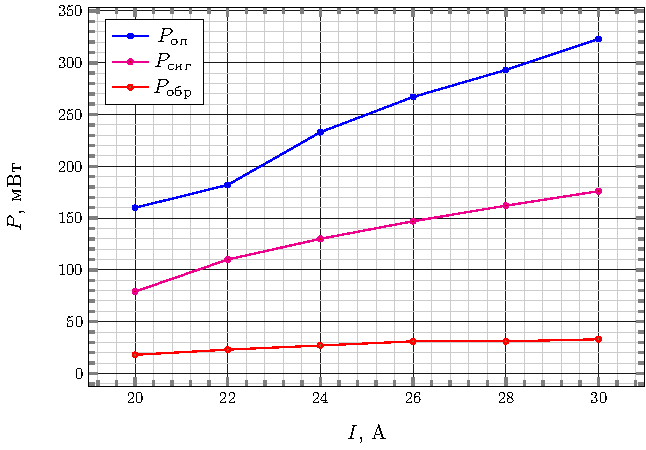
\includegraphics[]{fig/fig}
	\caption{Мощность опорного пучка, сигнального и обращённого}
	\label{fig:1}
\end{figure}



\section{Задания}
\subsection{Время релаксации}
Рассчитаем теоретически время релаксации показателя преломления в пропускающей решетке по формуле
\begin{equation}
	\tau_{r}=\frac{\tau_{0}}{1+4 \chi k_{x}^{2} \tau_{0}} = 7.11 \cdot 10^{-4} \text{ с}.
\end{equation}
где $\tau_0 = 16\cdot10^{-4}$ c, $\chi = 10^{-7}$ м${^2}$/c, $k_x = \frac{2\pi}{\lambda}\sin\frac{\theta}{2}$, $\lambda = 1064 \cdot 10^{-9}$ м, $\theta \approx 5/330$ рад.

\subsection{Коэффициент отражения}
Считая $\sigma_0 \sim (1\divisionsymbol 10) \cdot 10^{-10}$ Сименс/м (что в СГС порядка единицы),  рассчитываем интенсивность из известных экспериментальных условий как
\begin{equation}
	I_0 = \frac{2 P_\text{оп}}{S_\text{пучка}}, \qq{где} S_\text{пучка}=\pi\qty(\frac{d_\text{пучка}}{2})^2.
\end{equation}
Здесь $d=0.1$ см, $L$ приведено к безразмерному виду преобразованием $L' = L\cdot k^2 / k_z \varepsilon_0$, и для разных входных мощностей (токов накачки) посчитаны значения коэффициента отражения $r^2 = \tg^2(G\cdot l)$. В $G$ взяты значения $\epsilon_0 = \sqrt{n}  = \sqrt{1.5}$, $\rho_0 C_p\approx 10^7$ эрг/см${}^3$К, $\qty(\pdv{\varepsilon}{T})_p\approx 10^{-3}$ K${}^{-1}$. Полученные значения  предоставлены на графике ниже.
\begin{figure}[H]
	\centering
	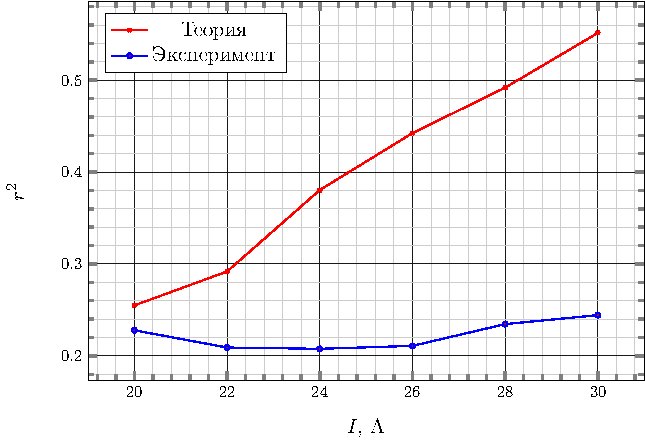
\includegraphics[]{fig/fig2}
	\caption{Коэффициент отражения}
	\label{fig:2}
\end{figure}

Как видно, теоретическое значение коэффициента растет с ростом накачки, что отвечает связи $r \sim \tg P$. Экспериментальные значения меньше. Во-первых, теоретическая формула получена в ряде приближений, например, слабого поглощения. В реальности поглощение может привести к уменьшению мощности сигнального пучка, и, соответственно, коэффициента ОВФ-отражения. Кроме того, могут быть экспериментальные особенности установки: например, возникновение при нагреве активной среды лазера тепловой линзы что приводит к появлению паразитных мод в лазере, увеличению угла расходимости лазернго пучка. Недостаточная термостабилизация элементов установки может привести к разбросу характеристик, таких как длина генерируемой волны, мощность пучка - и в итоге частично подавлять ОВФ-эффект.

\newpage
\addcontentsline{toc}{section}{Заключение}
\section*{Заключение}
В настоящей работе мы изучили метод преобразования излучения четырехволновым взаимодействием, рассчитали коэффициент отражения ОВФ-зеркала, получили зависимости мощностей трех пучков от тока накачки. Качественно наблюдается рост коэффициента ОВФ-отражения при росте мощности накачки, хотя количественно в теории обращённый фронт мог бы быть более мощным: но за счет существенной неидеальности лабораторных условий, приводящих к возникновению побочных эффектов - таких, как искажение модового состава лазерного излучения, увеличение угла пучка излучения и так далее - практическое значение меньше теоретического. 

\begin{thebibliography}{}
  \bibitem{met} Миловский Н.\,Д., Мартынова О.\,В., Зиновьев А.\,П. Преобразование лазерного излучения методами нелинейной оптики: методическое пособие. -- Нижний Новгород: Нижегородский государственный университет им. Н.И. Лобачевского, 2014. -- 38 с.
    
\end{thebibliography}

\end{document}